%%%%%%%%%%%%%%%%%%%%%%%%%%%%%%%%%%%%%%%%%
% Beamer Presentation
% LaTeX Template
% Version 1.0 (10/11/12)
%
% This template has been downloaded from:
% http://www.LaTeXTemplates.com
%
% License:
% CC BY-NC-SA 3.0 (http://creativecommons.org/licenses/by-nc-sa/3.0/)
%
%%%%%%%%%%%%%%%%%%%%%%%%%%%%%%%%%%%%%%%%%

%----------------------------------------------------------------------------------------
%	PACKAGES AND THEMES
%----------------------------------------------------------------------------------------

\documentclass[UTF8,aspectratio=169,14pt]{ctexbeamer}

\usepackage{hyperref}
\hypersetup{
	colorlinks=true,
	linkcolor=red,
	anchorcolor=blue,
	citecolor=green
}

\mode<presentation> {
	
	% The Beamer class comes with a number of default slide themes
	% which change the colors and layouts of slides. Below this is a list
	% of all the themes, uncomment each in turn to see what they look like.
	
	%\usetheme{default}
	%\usetheme{AnnArbor}
	%\usetheme{Antibes}
	%\usetheme{Bergen}
	%\usetheme{Berkeley}
	%\usetheme{Berlin}
	%\usetheme{Boadilla}
	%\usetheme{CambridgeUS}
	%\usetheme{Copenhagen}
	%\usetheme{Darmstadt}
	%\usetheme{Dresden}
	%\usetheme{Frankfurt}
	%\usetheme{Goettingen}
	%\usetheme{Hannover}
	%\usetheme{Ilmenau}
	%\usetheme{JuanLesPins}
	%\usetheme{Luebeck}
	\usetheme{Madrid}
	%\usetheme{Malmoe}
	%\usetheme{Marburg}
	%\usetheme{Montpellier}
	%\usetheme{PaloAlto}
	%\usetheme{Pittsburgh}
	%\usetheme{Rochester}
	%\usetheme{Singapore}
	%\usetheme{Szeged}
	%\usetheme{Warsaw}
	
	% As well as themes, the Beamer class has a number of color themes
	% for any slide theme. Uncomment each of these in turn to see how it
	% changes the colors of your current slide theme.
	
	%\usecolortheme{albatross}
	%\usecolortheme{beaver}
	%\usecolortheme{beetle}
	%\usecolortheme{crane}
	%\usecolortheme{dolphin}
	%\usecolortheme{dove}
	%\usecolortheme{fly}
	%\usecolortheme{lily}
	%\usecolortheme{orchid}
	%\usecolortheme{rose}
	%\usecolortheme{seagull}
	%\usecolortheme{seahorse}
	%\usecolortheme{whale}
	%\usecolortheme{wolverine}
	
	%\setbeamertemplate{footline} % To remove the footer line in all slides uncomment this line
	%\setbeamertemplate{footline}[page number] % To replace the footer line in all slides with a simple slide count uncomment this line
	
	%\setbeamertemplate{navigation symbols}{} % To remove the navigation symbols from the bottom of all slides uncomment this line
}

\usepackage{graphicx} % Allows including images
\graphicspath{{./figs/}}
\usepackage{booktabs} % Allows the use of \toprule, \midrule and \bottomrule in tables
\usepackage{longtable}
\usepackage{listings}
\usepackage{xcolor}
\lstset{numbers=left, %设置行号位置
	numberstyle=\tiny, %设置行号大小
	keywordstyle=\color{blue}, %设置关键字颜色
	commentstyle=\color[cmyk]{1,0,1,0}, %设置注释颜色
	frame=single, %设置边框格式
	escapeinside=``, %逃逸字符(1左面的键),用于显示中文
	%breaklines, %自动折行
	extendedchars=false, %解决代码跨页时,章节标题,页眉等汉字不显示的问题
	xleftmargin=2em,xrightmargin=2em, aboveskip=1em, %设置边距
	tabsize=4, %设置tab空格数
	showspaces=false %不显示空格
}
% Fonts
% \usepackage{libertine}
% \setmonofont{Courier}
\setCJKsansfont[ItalicFont=Noto Serif CJK SC Black, BoldFont=Noto Sans CJK SC Black]{Noto Sans CJK SC}


%----------------------------------------------------------------------------------------
%	TITLE PAGE
%----------------------------------------------------------------------------------------

\title[第2讲]{第2讲 :操作系统与系统结构和程序设计语言} % The short title appears at the bottom of every slide, the full title is only on the title page
\subtitle{第三节:RISC-V的系统编程}
\author{向勇、陈渝} % Your name
\institute[清华大学] % Your institution as it will appear on the bottom of every slide, may be shorthand to save space
{
清华大学计算机系 \\ % Your institution for the title page
\medskip
\textit{xyong,yuchen@tsinghua.edu.cn} % Your email address
}
\date{\today} % Date, can be changed to a custom date

\begin{document}

\begin{frame}
\titlepage % Print the title page as the first slide
\end{frame}

\begin{frame}
\frametitle{提纲} % Table of contents slide, comment this block out to remove it
\tableofcontents % Throughout your presentation, if you choose to use \section{} and \subsection{} commands, these will automatically be printed on this slide as an overview of your presentation
\end{frame}

%----------------------------------------------------------------------------------------
%	PRESENTATION SLIDES
%----------------------------------------------------------------------------------------

%------------------------------------------------
\section{第三节:RISC-V的系统编程 } % Sections can be created in order to organize your presentation into discrete blocks, all sections and subsections are automatically printed in the table of contents as an overview of the talk
%------------------------------------------------

\subsection{高级语言编译到机器指令} % A subsection can be created just before a set of slides with a common theme to further break down your presentation into chunks
\subsection{理解stack}


\begin{frame}
	\frametitle{高级语言}
	\framesubtitle{系统编程语言}

\begin{itemize}
	
	\item 对当前编程语言的理解
	\begin{itemize}
		\item 系统编程语言(system language)定义现在似乎没有特别严谨和一致的定义
		\item 系统编程语言用于构建控制底层计算机硬件的软件系统,并提供由用于构建应用程序和服务的更高级应用程序编程语言使用的软件平台。
		\item 开发操作系统的系统编程语言其实很多;还离不开汇编语言。
	\end{itemize}
	\centering
	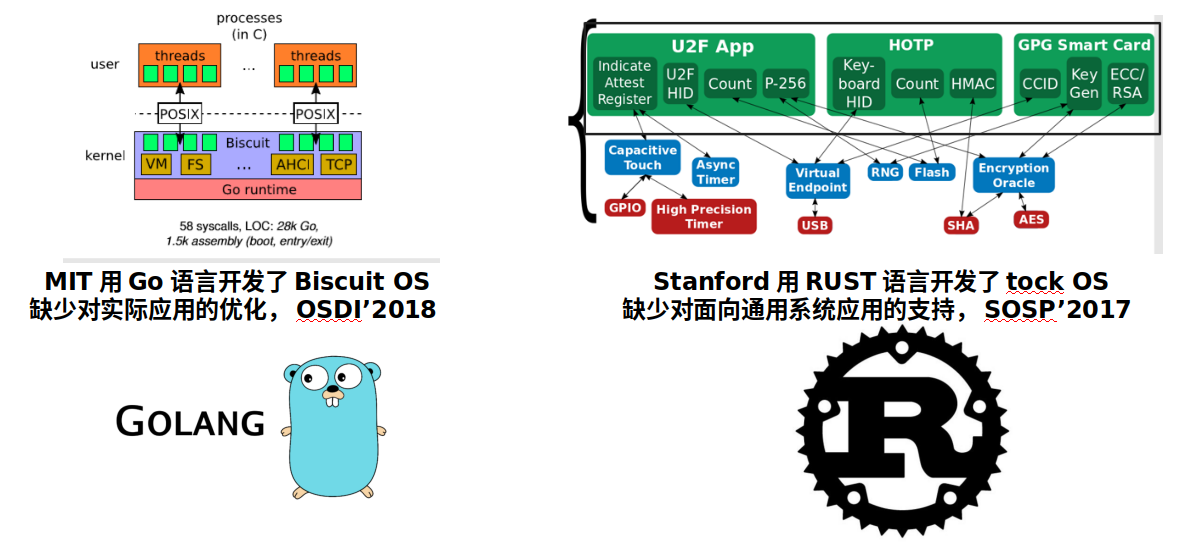
\includegraphics[width=0.7\linewidth]{go-rust-4-os}
\end{itemize}	
\end{frame}

\begin{frame}
	\frametitle{高级语言}
	\framesubtitle{Why Rust}
	
	\begin{itemize}
		
		\item Why Rust?
		\begin{itemize}
			\item CS140e:Stanford 实验性课程,Rust OS for Raspi3
			\item RVirt:MIT RISC-V Hypervisor
			\item Writing an OS in Rust —— BlogOS:详尽的 Rust OS 教程
			\item 产业界: 蚂蚁金服:Occlum  -- Facebook:Libra
		\end{itemize}

	\end{itemize}	
	
\end{frame}


\begin{frame}
	\frametitle{高级语言}
	\framesubtitle{Why Rust}
	
	\begin{itemize}
		
		\item Rust 的主要特性
		\begin{itemize}
			\item 内存+线程安全
			\item 高级语言特性
			\item 成熟的工具链
			\item 友好的助教+社区(OS示例代码+文档)生态
			\item 学习Rust的入门门槛比较高(认清你自己,量力而行)
		\end{itemize}
		
	\end{itemize}	
	
\end{frame}





\begin{frame}[fragile]
	\frametitle{高级语言编译到机器指令}
	\framesubtitle{C/Rust代码}

	\begin{columns}[t]
	\begin{column}{.45\linewidth}
		
%\small	
%\begin{lstlisting}[language = C]
\begin{block}{}
\begin{verbatim}
//C CODE
int sum_to(int n) {
  int acc = 0;
  for (int i = 0; i < n; i++) {
    acc += i;
  }
  return acc;
}
\end{verbatim}
\end{block}
%\end{lstlisting}
\end{column}

\begin{column}{.45\linewidth}
\begin{block}{}
\begin{verbatim}
//Rust CODE
fn sum_to(n:i32)->i32 {
  let mut acc = 0;
  for i in 0..n {
    acc += i;
  }
  从acc
}
\end{verbatim}
\end{block}
\end{column}
\end{columns}
	
\end{frame}





%\begin{frame}[fragile]
%	\frametitle{高级语言编译到机器指令}
%	\framesubtitle{Rust代码}
%	
%\small
%%\begin{lstlisting}[language = C]
%\begin{verbatim}
%fn sum_to(n:i32)->i32 {
%  let mut acc = 0;
%  for i in 0..n {
%    acc += i;
%  }
%  acc
%}
%\end{verbatim}
%%\end{lstlisting}
%	
%\end{frame}

\begin{frame}[fragile,plain]
\frametitle{高级语言编译到机器指令}
\framesubtitle{汇编代码}

\small	
%\begin{lstlisting}
\centering
\begin{block}{}
\begin{verbatim}
# sum_to(n)
# expects argument in a0
# returns result in a0
sum_to:
mv t0, a0          # t0 <- a0
li a0, 0           # a0 <- 0
loop:
add a0, a0, t0     # a0 <- a0 + t0
addi t0, t0, -1    # t0 <- t0 - 1
bnez t0, loop      # if t0 != 0: pc <- loop
ret
\end{verbatim}
\end{block}
%\end{lstlisting}	

\begin{itemize}
	
	\item 有限的抽象
	\begin{itemize}
	  \item 无类型的位置参数 -- 没有局部变量 -- 仅寄存器
	\end{itemize}
		
\end{itemize}
	
\end{frame}

\begin{frame}[plain]
	
	\frametitle{高级语言编译到机器指令}
	\framesubtitle{RISC-V寄存器}	
	\begin{table}[h]
		\caption{RISC-V寄存器描述}\small
		\begin{tabular}{|l|l|l|l|}
			\hline
			Register & ABI Name & Description                      & Saver  \\\hline
			x0       & zero     & Hard-wired zero                  & ------ \\\hline
			x1       & ra       & Return address                   & Caller \\\hline
			x2       & sp       & Stack pointer                    & Callee \\\hline
			x3       & gp       & Global pointer                   & ------ \\\hline
			x4       & tp       & Thread pointer                   & ------ \\\hline
			x5-7     & t0-2     & Temporaries                      & Caller \\\hline
			x8       & s0/fp    & Saved register/frame pointer     & Callee \\\hline
			x9       & s1       & Saved register                   & Callee \\\hline
			x10-11   & a0-1     & Function arguments/return values & Caller \\\hline
			x12-17   & a2-7     & Function arguments               & Caller \\\hline
			x18-27   & s2-11    & Saved registers                  & Callee \\\hline
			x28-31   & t3-6     & Temporaries                      & Caller \\
			\hline
		\end{tabular}
	\end{table}
	
\end{frame}

\begin{frame}[fragile]
\frametitle{高级语言编译到机器指令}
\framesubtitle{汇编代码}
	
\begin{itemize}
	
	\item 机器甚至看不到汇编代码
	\item 查看机器指令的二进制编码
	\begin{itemize}
		\item 每条指令:16位或32位
		\item 例如`mv t0,a0`编码为0x82aa
		\item 从asm不太完全一对一编码(但是很接近)
	\end{itemize}
	
	\item 另一个函数将如何调用sum\_to?
\end{itemize}	

\begin{lstlisting}
main:
  li a0, 10          # a0 <- 10
  call sum_to
\end{lstlisting}

	
\end{frame}

\begin{frame}[fragile]
\frametitle{高级语言编译到机器指令}
\framesubtitle{汇编代码}
	
\begin{itemize}
	
	\item 函数调用的语义是什么?	


%\begin{lstlisting}
\begin{block}{}
\begin{verbatim}
call label :=
  ## ra <- address of next instruction
  ra <- pc + 4       ;
  ## jump to label
  pc <- label        ; 
\end{verbatim}
\end{block}  
%\end{lstlisting}
\item 机器不理解标签
\item 换为相对于PC的跳转或绝对跳转	
\end{itemize}

\end{frame}




\begin{frame}[fragile]
	\frametitle{高级语言编译到机器指令}
	\framesubtitle{汇编代码}
	
	\begin{itemize}
		
		\item 函数返回(return)的语义是什么??	
		
		
%		\begin{lstlisting}
\begin{block}{}
\begin{verbatim}
ret :=  pc <- ra
看看汇编代码: demo1.S
(gdb) file user/_demo1
(gdb) break main
(gdb) continue
(gdb) layout split
(gdb) stepi
(gdb) info registers\begin{itemize}
(gdb) p $a0
(gdb) advance 18
(gdb) si
(gdb) p $a0
\end{verbatim}
\end{block}  
%\end{lstlisting}

	\end{itemize}
	
\end{frame}



\begin{frame}
	\frametitle{高级语言编译到机器指令}
\framesubtitle{调用约定}
	
 \begin{itemize}
	\item 如何传递参数?
	\begin{itemize}
	 	\item a0,a1,...,a7,放在堆栈上
	\end{itemize}
	\item 值如何返回?
	\begin{itemize}
		\item a0,a1
	\end{itemize}	
	\item 谁保存寄存器?
	\begin{itemize}
		\item 指定为已保存的呼叫者或被呼叫者
	    \item ra可以是保存被呼叫者的寄存器吗
    \end{itemize}   
	
	\item 汇编代码应遵循此约定
	\item GCC生成的C代码遵循此约定
	\item RUST代码遵循此约定
	\item 这意味着各种代码之间都可以互操作

\end{itemize} 
	% s0 / fp是怎么回事?
	% 我们使用-fno-omit-frame-pointer进行编译
	
\end{frame}


\begin{frame}[fragile,plain]
	\frametitle{高级语言编译到机器指令}
	\framesubtitle{Stack Frames}
\small 
%\begin{lstlisting}
%\begin{block}{}
%\begin{verbatim}
%Stack
%.
%.
%+->          .
%|   +-----------------+   |
%|   | return address  |   |
%|   |   previous fp ------+
%|   | saved registers |
%|   | local variables |
%|   |       ...       | <-+
%|   +-----------------+   |
%|   | return address  |   |
%+------ previous fp   |   |
%| saved registers |   |
%| local variables |   |
%+-> |       ...       |   |
%|   +-----------------+   |
%|   | return address  |   |
%|   |   previous fp ------+
%|   | saved registers |
%|   | local variables |
%|   |       ...       | <-+
%|   +-----------------+   |
%|   | return address  |   |
%+------ previous fp   |   |
%| saved registers |   |
%| local variables |   |
%$fp --> |       ...       |   |
%+-----------------+   |
%| return address  |   |
%|   previous fp ------+
%| saved registers |
%$sp --> | local variables |
%+-----------------+
%\end{verbatim}
%\end{block} 
%\end{lstlisting}	
	
%\begin{figure}
	\centering
	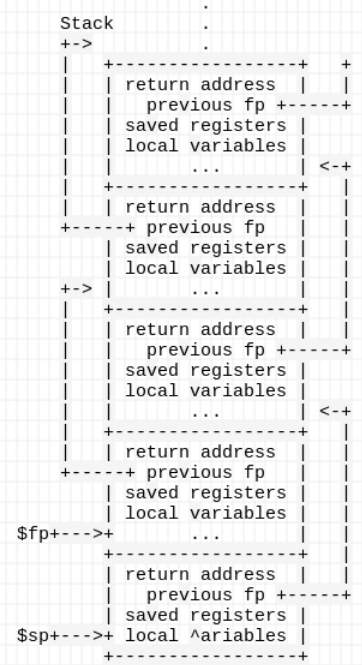
\includegraphics[width=0.25\linewidth]{stack}
	
	%http://asciiflow.com/
%	\caption{函数栈}
%\end{figure}
	
\end{frame}

%----------------------------------------------------------------------------------------

\end{document}
